\section{Heap Allocation}
\label{sec:res:heap}
In this section we consider a small experiment to investigate possible differences in heap fragmentation caused by dynamic allocation in {\C} and {\rust}.
The conducted experiment is a simple program which \textbf{1)} allocates 128 objects on the heap, and \textbf{2)} replaces one object picked at random 1024 times.
The objects are of the three sizes given in \autoref{tab:heap:objects}.

\begin{table}[H]
  \centering
  \begin{tabular}{l|c|l}
    \textbf{Name} & \textbf{Size (32-bit words)} & \textbf{Color} \\
    \hline
    A & 2 & Green \\
    B & 3 & Red \\
    C & 6 & Blue \\
    \hline
  \end{tabular}
  \caption{Object sizes}
  \label{tab:heap:objects}
\end{table}

The heap allocation pattern was recorded after the first phase of the program, and are given in \autoref{fig:heap:init}.
The figure shows a two-dimentional plot of the memory layout with address \mem{0} at the top left corner, and the top row represents the addresses \mem{0} through \mem{63}.
We see that the initial allocation pattern is alternating between these three object sizes, and the white spaces between are padding, due to alignment rules of the allocator.
The objects are created in the same order in both {\C} and {\rust} and we see that the allocation patterns are identical.

\begin{figure}[H]

  \centering
  \begin{subfigure}{0.47\textwidth}
    \centering
    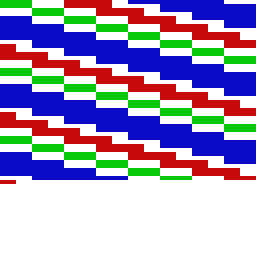
\includegraphics[scale=0.15]{results/plots/heap/cinit}
    \caption{C}
    \label{fig:heap:init:c}
  \end{subfigure}
  \hfill
  \begin{subfigure}{0.47\textwidth}
      \centering
    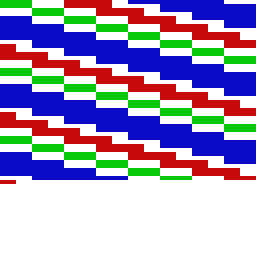
\includegraphics[scale=0.15]{results/plots/heap/rinit}
    \caption{Rust}
    \label{fig:heap:init:r}
  \end{subfigure}
  \caption{Initial heap allocation of 128 objects in {\rust} and {\C}}
  \label{fig:heap:init}

\end{figure}

To get comparable results for both {\C} and {\rust} the pseudo randomly picked objects, are the same.
This is controlled by using the same random number generator, for both languages (this is the same \gls{rng} as discussed in \autoref{sec:res:perf}).
\autoref{fig:heap:frag} presents the heap allocation pattern after the second phase has been executed.
From this figure, we see that the allocation patterns in {\rust} and {\C} are identical.

\begin{figure}[H]

  \centering
  \begin{subfigure}{0.47\textwidth}
    \centering
    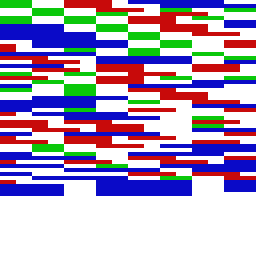
\includegraphics[scale=0.15]{results/plots/heap/cfrag}
    \caption{C}
    \label{fig:heap:frag:c}
  \end{subfigure}
  \hfill
  \begin{subfigure}{0.47\textwidth}
      \centering
    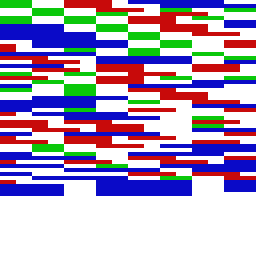
\includegraphics[scale=0.15]{results/plots/heap/rfrag}
    \caption{Rust}
    \label{fig:heap:frag:r}
  \end{subfigure}
  \caption{Heap allocation after processing in {\rust} and {\C}}
  \label{fig:heap:frag}

\end{figure}
